\begin{figure}
    \centering
    \setlength{\resLen}{1.06in}
    \setlength{\raiseLen}{0.9in}
    \addtolength{\tabcolsep}{-3.5pt}
    \small
    %
    \begin{tabular}{ccc}
        \begin{overpic}[width=\resLen]{images/lucy/color_aniso_x.jpg}
            \put(2,2){\color{white} \bfseries x}
        \end{overpic} &
        \begin{overpic}[width=\resLen]{images/lucy/color_aniso.jpg}
            \put(2,2){\color{white} \bfseries y}
        \end{overpic} &
\\
        \textbf{(a) Multi.} & \textbf{(b) 400nm} & \textbf{(c) 550nm} & \textbf{(d) 700nm}
    \end{tabular}
    \caption{\label{fig:multiwave_aniso}
        \gy{(a)~Multi-spectral rendering of an anisotropic ($y$-axis) media by 100 particles with radii 300nm.
        (b--d)~Monochrome renderings of the same model at three wavelengths.}
    }
\end{figure}


% 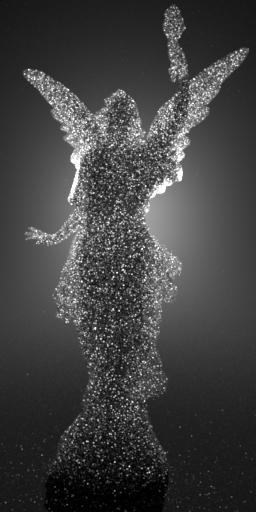
\includegraphics[width=\resLen]{images/lucy/color_aniso_x_400nm.jpg} &
% 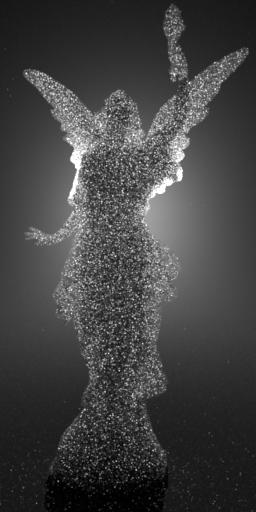
\includegraphics[width=\resLen]{images/lucy/color_aniso_x_550nm.jpg} &
% 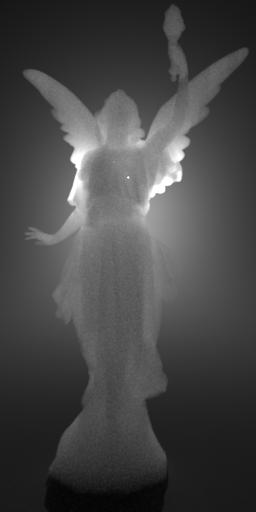
\includegraphics[width=\resLen]{images/lucy/color_aniso_x_700nm.jpg} 